%
%   N K Y M
%    A A A A
%

%   this file is "nkym.tex"

\documentclass[10pt,b5paper,papersize,dvipdfmx]{jsbook}

\usepackage{vuccaken}
\usepackage{vuccaken2019}

\begin{document} % 以下本文

% - - - - - - - - - - - - - - - - - - - - - - - - %
\kaishititle%
  {こてんりきがくではない}% title
  {物理科学科4回生}% 所属
  {中山 敦貴}% name
% - - - - - - - - - - - - - - - - - - - - - - - - %

% \setcounter{tocdepth}{2} % 目次にどこまで表示するか
% \tableofcontents % 目次出力
% \clearpage % 改ページ

進捗報告会のときの進捗をコピペしました。\par
ゼミ終わったら本気出す!!!

% - - - - - - - - - - - - - - - - - - - - - - - - %
\section*{はじめに}
% - - - - - - - - - - - - - - - - - - - - - - - - %
とりあえず、内容としましては、古典力学で仮定されていた局所実在論では説明できないようなことが量子の世界では起こっているという話をします。
具体的には、局所実在論であれば必ず成立するベルの不等式が、エンタングルメントという量子論特有の性質を持った系では破れることがあるということを示します。\par
章立ては大きくは以下のような感じだと思います。


% - - - - - - - - - - - - - - - - - - - - - - - - %
\section{局所実在論}
% - - - - - - - - - - - - - - - - - - - - - - - - %

% - - - - - - - - - - - - - - - - - - - - - - - - %
\section{ベルの不等式}
% - - - - - - - - - - - - - - - - - - - - - - - - %

%
\subsection{光子の偏光}

定義:
(光子の)電場の振動の方向を偏光と呼ぶ。

\begin{figure}[ht]
  \centering
  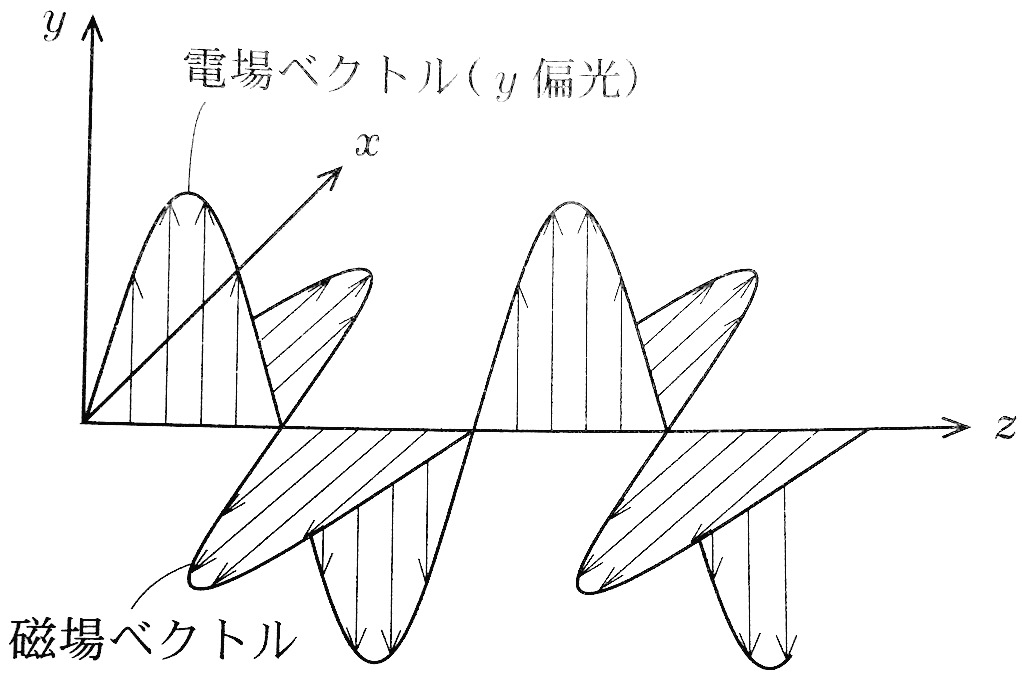
\includegraphics[width=40mm]{nkym/fig/henkou.jpeg}
  % \caption{軸の設定。(参考文献[1], P.26)}
  % \label{}
\end{figure}

偏光子を通過した後の光子の偏光は、偏光子の偏光軸と一致する。

光子が偏光子を通過する確率は、光子と偏光子の偏光軸のなす角を$\theta$として
\begin{align*}
  P(\theta) = \frac12 \cos^2\theta
\end{align*}

%
\subsection{ベルの不等式}

表のように$x, \theta, \phi$の3列に$+, -$を割り振るゲームを考える。
この表の中で$x$と$\phi$にそれぞれ$+$があるものの個数を$n(x=+,\phi=+)$のように書くと、次の不等式が必ず成り立つ:
\begin{align*}
  n(x=+,\phi=+) + n(\phi=-,\theta=+) \ge n(x=+,\theta=+).
\end{align*}

\begin{table}[htbp]
  \centering
  \caption{$+, -$の割り振り}
  \begin{tabular}{ccc} \hline
    $x$ & $\theta$ & $\phi$ \\ \hline
    $+$ & $+$ & $-$ \\
    $-$ & $+$ & $+$ \\
    $\vdots$ & $\vdots$ & $\vdots$ \\ \hline
  \end{tabular}
\end{table}

\noindent 証明:\par
前の表において$n(x=+,\phi=+)$は$\theta = +$と$\theta = -$の和である。
\begin{align}
  \label{eq:bell-1}
  n(x=+,\phi=+) = \textcolor{red}{n(x=+,\phi=+, \theta=+)} + n(x=+,\phi=+, \theta=-).
\end{align}
同様にして
\begin{align}
  \label{eq:bell-2}
  n(\phi=-,\theta=+) &= \textcolor{blue}{n(x=+, \phi=-,\theta=+)} + n(x=-, \phi=-,\theta=+)
  , \\
  \label{eq:bell-3}
  n(x=+,\theta=+) &= \textcolor{red}{n(x=+, \phi=+, \theta=+)} + \textcolor{blue}{n(x=+, \phi=-, \theta=+)}.
\end{align}
\siki{bell-1}と\siki{bell-2}の和と\siki{bell-3}を比較すると、\siki{bell-1}と\siki{bell-2}の第2項の分だけ\siki{bell-3}の方が小さい。よって、ベルの不等式
\begin{align*}
  n(x=+,\phi=+) + n(\phi=-,\theta=+) \ge n(x=+,\theta=+)
\end{align*}
が成り立つ。
\qed

%
\subsection{アスペの実験}

%
\subsubsection{Ca原子の放射光の検出}

Ca原子にレーザー光を照射して、特定のエネルギーレベルに励起させると、基底状態に戻る際に2個の互いに直交した偏光を持つ光子(緑色と紫色)が放出される。

図のような装置で2つの光子を検出する。

\begin{figure}[ht]
  \centering
  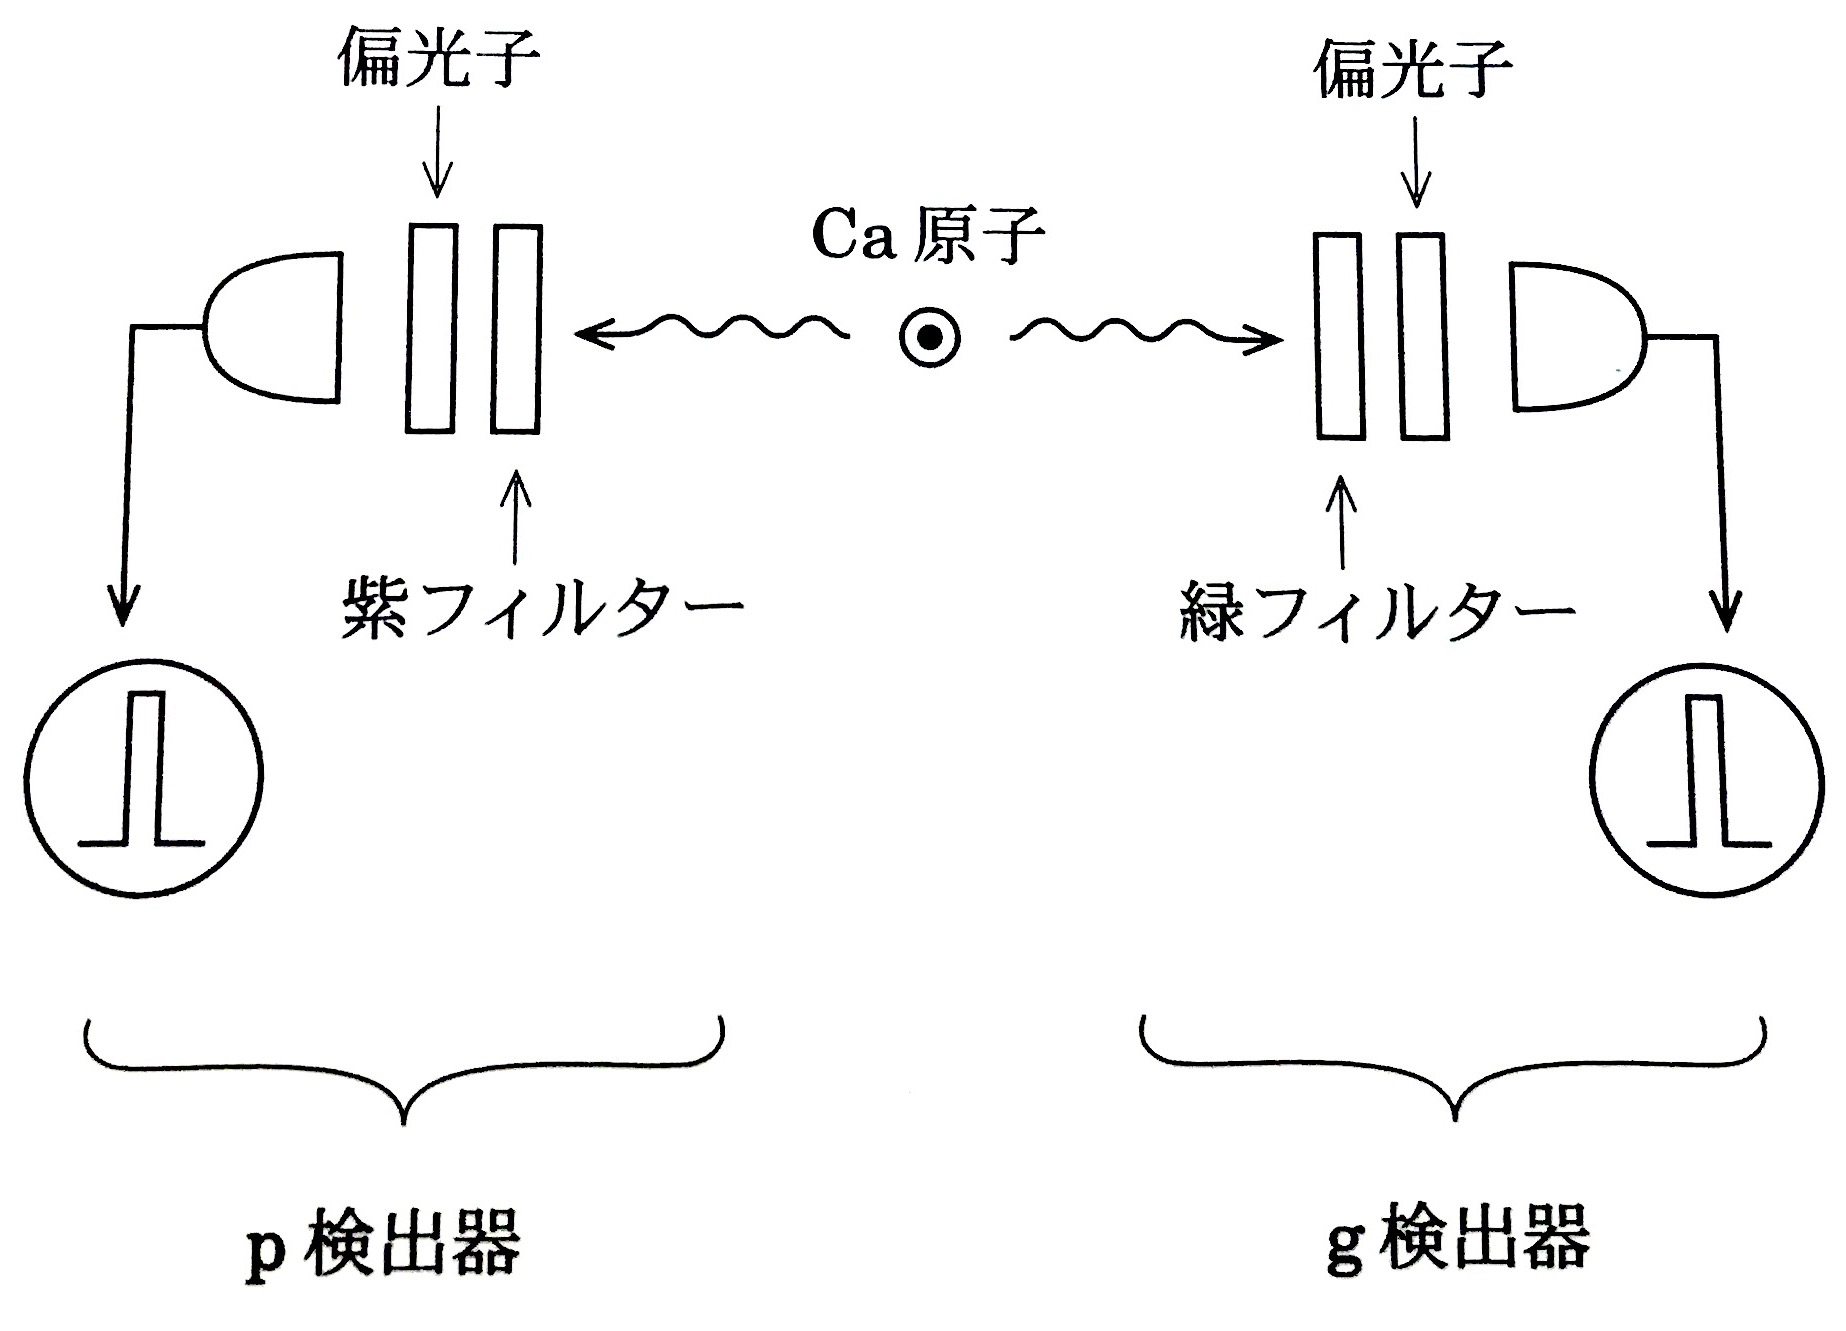
\includegraphics[height=40mm]{nkym/fig/souchi.jpeg}
  \caption{Ca原子から出た2つの光子の偏光を検出する装置。(参考文献[1], P.21)}
  % \label{}
\end{figure}

%
\subsubsection{検出器の偏光軸}

\begin{figure}[ht]
  \centering
  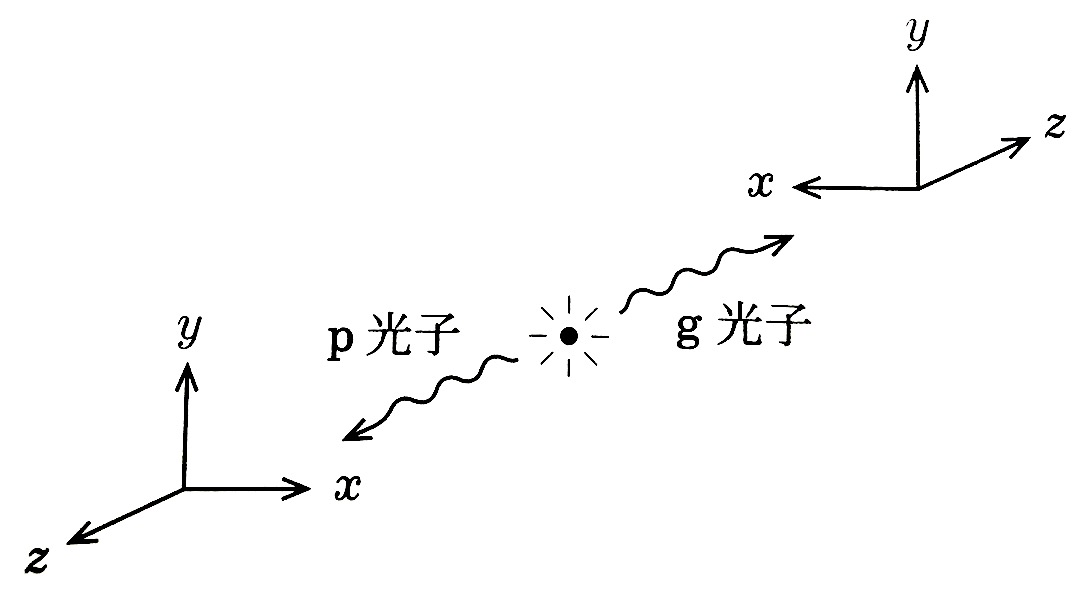
\includegraphics[width=40mm]{nkym/fig/zahyou-kei.jpeg}
  % \caption{軸の設定。(参考文献[1], P.26)}
  % \label{}
\end{figure}

光子の進行方向を$z$軸正の向きとし、水平方向に$x$軸、鉛直方向に$y$軸をとる。

p検出器とg検出器に付いている偏光子の偏光軸は、図のように、それぞれ2種類の設定を使う。

\begin{figure}[ht]
  \centering
  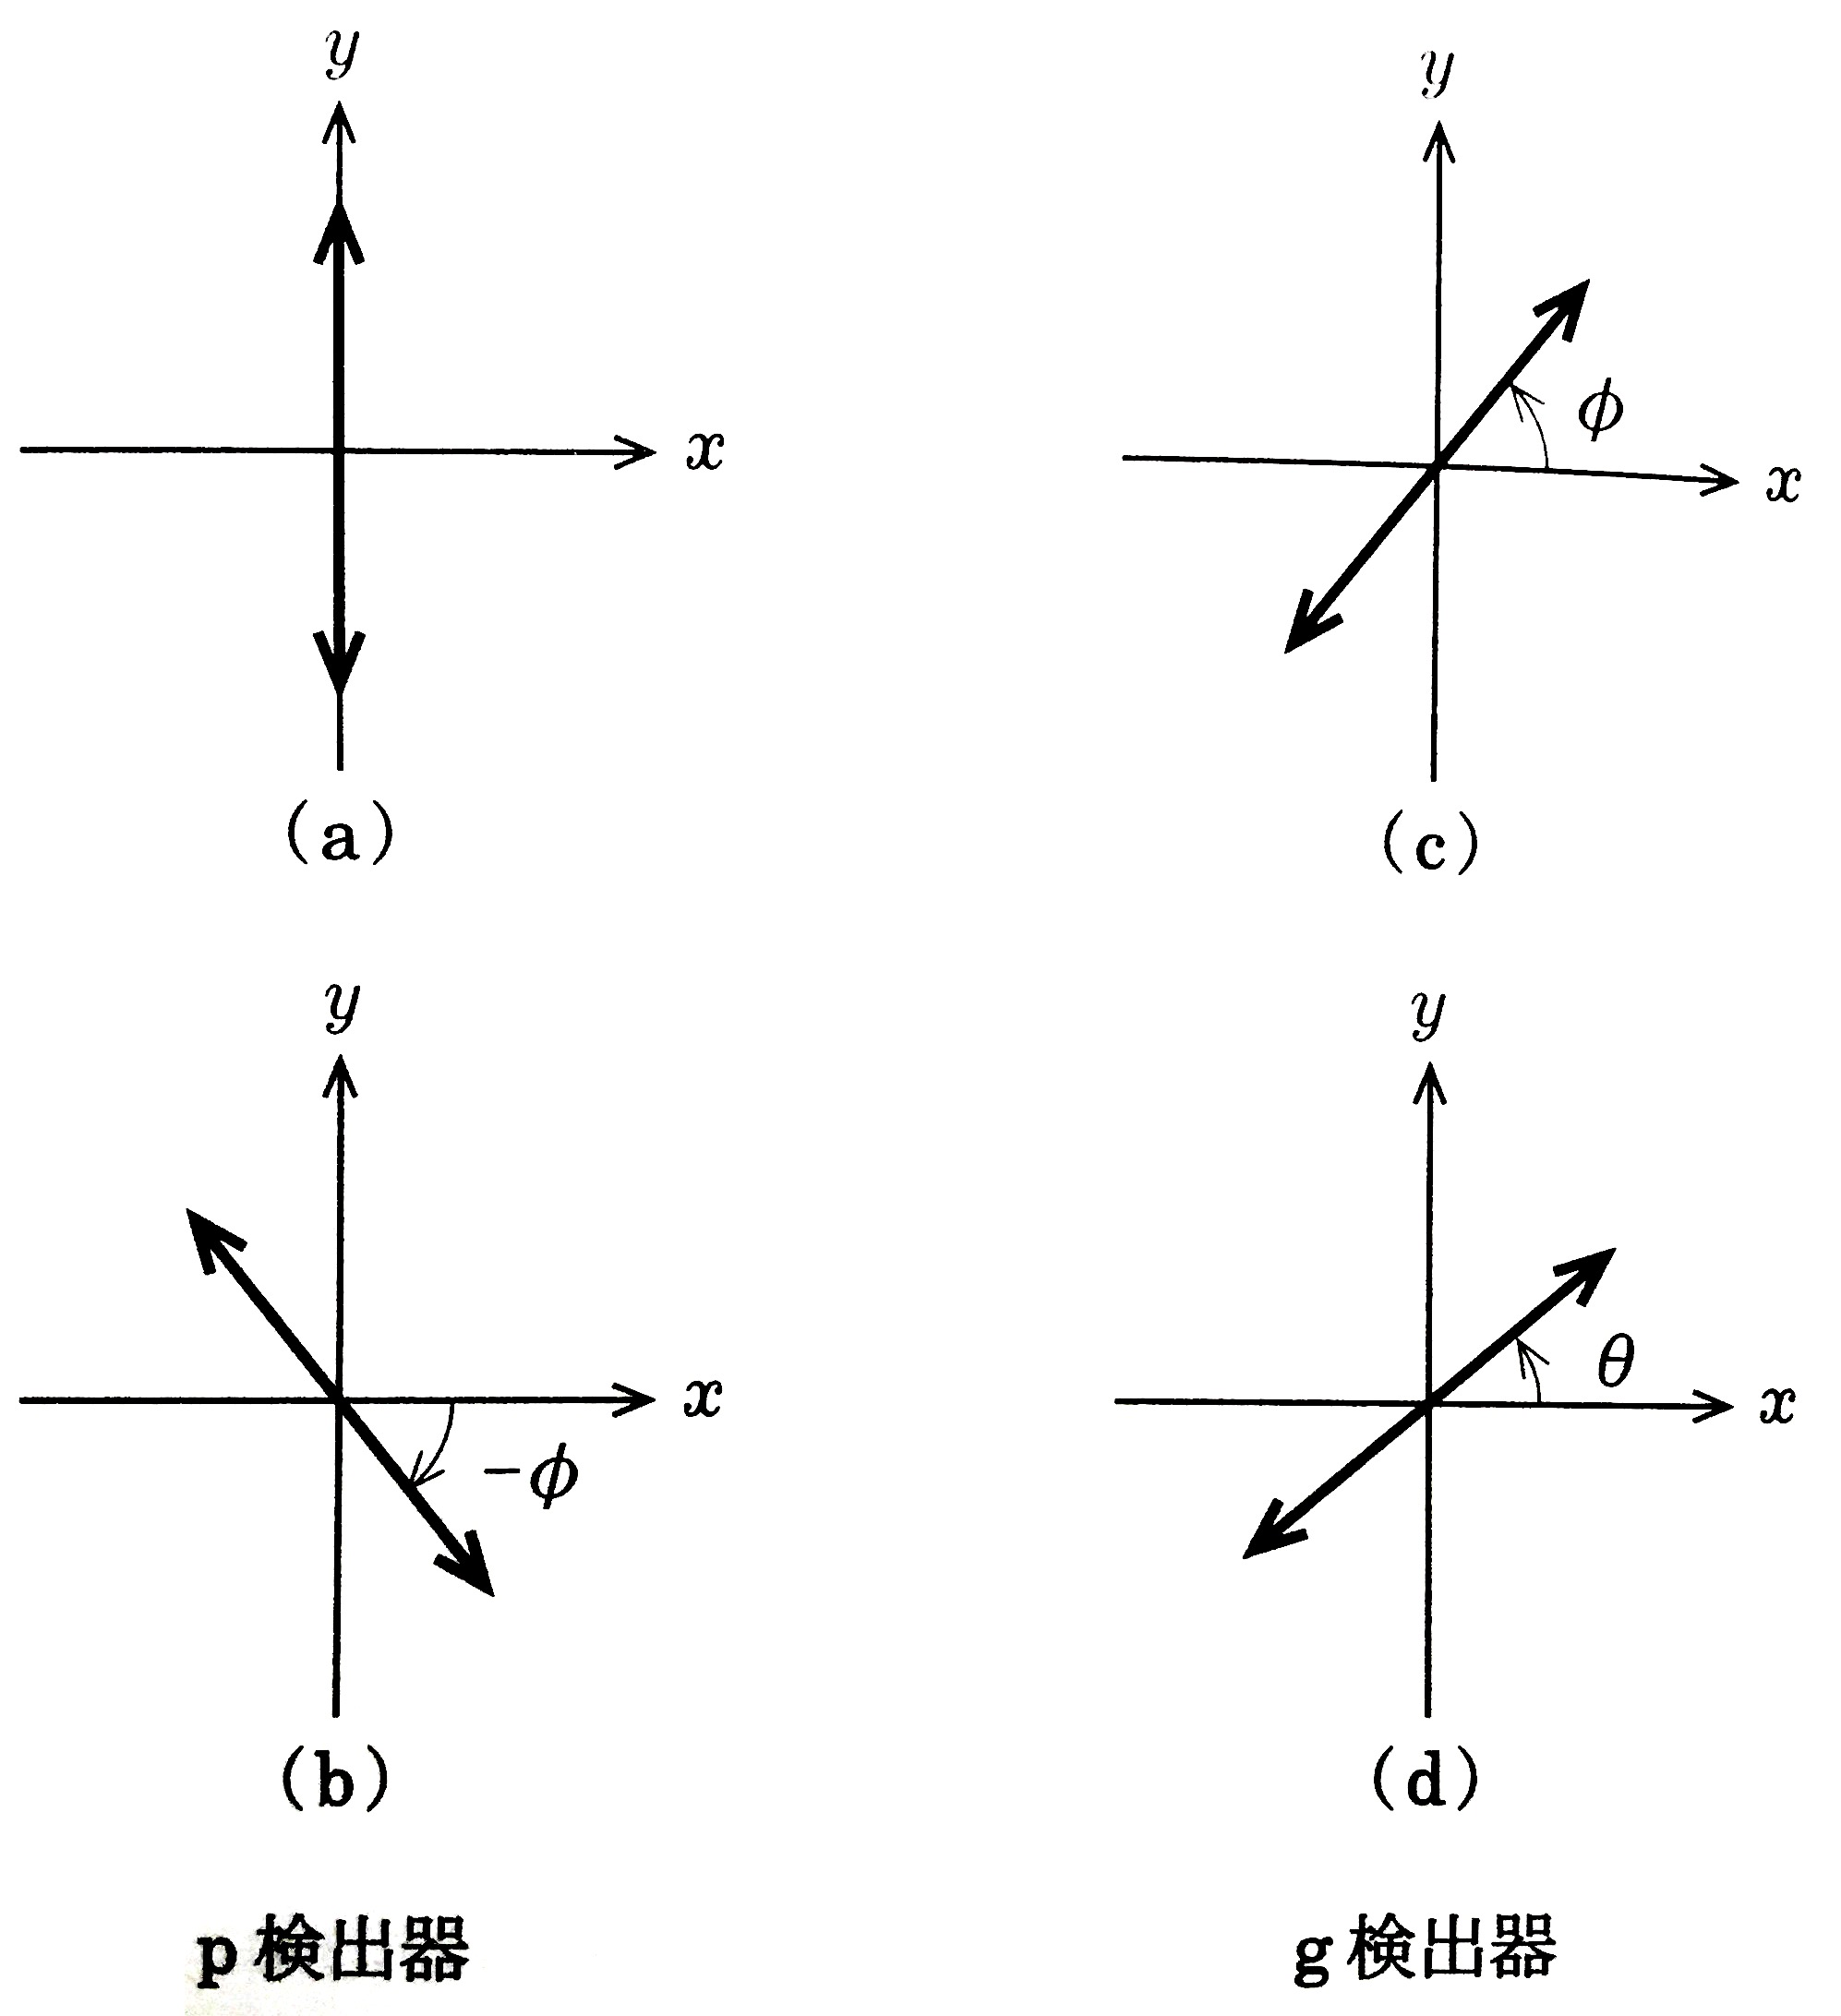
\includegraphics[width=45mm]{nkym/fig/henkou-jiku.jpeg}
  \caption{偏光軸の方向。(参考文献[1], P.26)}
  % \label{}
\end{figure}

%
\subsubsection{光子の測定}
p検出器の偏光子の偏光軸を$y$軸方向に、g検出器の偏光軸を$x$軸から$\phi$だけ回してセットし、単位時間あたりに両検出器が同時に光子を検出する回数$n(x=+,\phi=+)$を観測する。\par
同様にして、$n(x=+,\theta=+)$と$n(\phi=-,\theta=+)$を観測する。

単位時間当たりにp検出器が検出する光子の数を$N \,(\gg 1)$個として、
同時にg検出器が光子を検出する数を予想すると
\begin{align*}
  n(x=+,\phi=+) &= N \cos^2\phi, \\
  n(x=+,\theta=+) &= N \cos^2\theta, \\
  n(\phi=-,\theta=+) &= N \cos^2(\phi + \pi/2 - \theta) = N \sin^2(\phi - \theta).
\end{align*}

%
\subsubsection{ベルの不等式の破れ}

\begin{align*}
  \cos^2\phi + \sin^2(\phi - \theta) \ge \cos^2\theta.
\end{align*}
$\phi = 3\theta$とすると
\begin{align*}
  \cos^2 3\theta + \sin^2 2\theta - \cos^2\theta \ge 0.
\end{align*}
左辺を図示すると、$0 < \theta < 30^\circ$の範囲で不等式を満足していない。

実験してみると、この予想通りベルの不等式を満たさない場合がある。

\begin{figure}[htp]
  \centering
  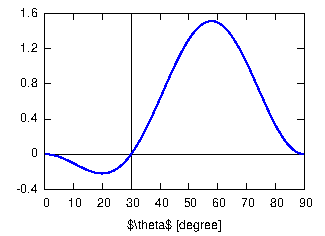
\includegraphics{nkym/fig/Aspect.pdf}
  \caption{不等式の左辺。}
  % \label{}
\end{figure}

\subsubsection{解釈}

\begin{itemize}
  \item 例えば$n(x=+,\phi=+)$を測定したとき、$\theta$が何であったかには言及していない(測定していない)。
  \item ベルの不等式を導く際は、$\theta$は隠れているだけで、$\theta=+$か$\theta=-$の事象が起きたはずだと仮定していた。
  \item 実はこの仮定が間違っており、3列に$+,-$を割り振るゲームと、アスぺの実験で考えた状況は異なるものであった。
\end{itemize}

つまり

\begin{itemize}
  \item 測定していない物理量は、常に確定(実在)しているとは限らない。
  \item アスぺの実験では、Ca原子から放出される2つの光子の偏光が互いに直交しているということがポイント。(エンタングルメント)
\end{itemize}

まとめ

\begin{itemize}
  \item 隠れた変数(理論)があれば、必ずベルの不等式を満たす。
  \item 偏光軸が直交した2つの光子(エンタングル状態)を用いた実験では、ベルの不等式を満たさない場合があることがわかった(アスぺの実験)。
  \item この実験結果は、隠れた変数理論(実在論)では記述できないような現象があることを示唆している。
  \item 周知の通り、量子力学では上のような現象も問題なく予測できる。つまり、量子力学は古典論を含み、かつ実在論を超えた理論である。
\end{itemize}


% - - - - - - - - - - - - - - - - - - - - - - - - %
\section{量子エンタングルメント}
% - - - - - - - - - - - - - - - - - - - - - - - - %

% - - - - - - - - - - - - - - - - - - - - - - - - %
\section{解釈?}
% - - - - - - - - - - - - - - - - - - - - - - - - %

% \begin{figure}[htbp]
%   \centering
%   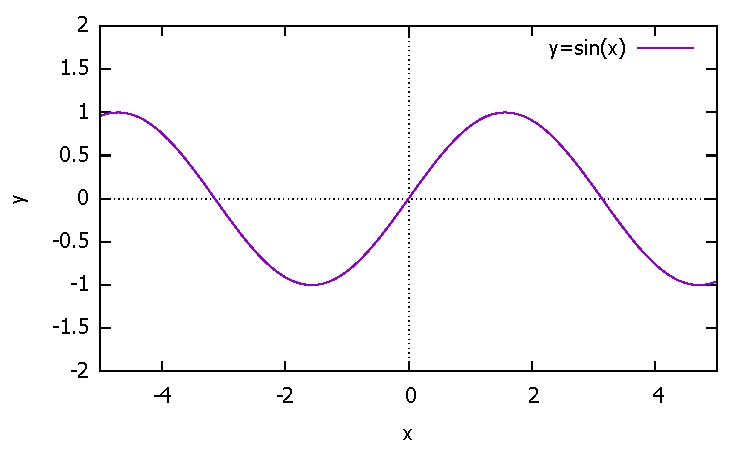
\includegraphics[width=10cm]{temp/fig-sin.pdf}
%   \caption{$y=\sin x$のグラフ。gnuplotで作成した。}
%   \label{fig:sin}
% \end{figure}

\clearpage

%% 参考文献
\begin{sanko}
  \begin{enumerate}
    \item 清水明、「新版 量子論の基礎」、サイエンス社、2004年。
    \item 清水明、スライド「EPRパラドックスからベルの不等式へ」\\
      \url{http://as2.c.u-tokyo.ac.jp/lecture_note/kstext04_ohp.pdf}
    \item J.J.サクライ、「現代の量子力学(上)」、吉岡書店。
    \item 森田邦久、「アインシュタイン vs. 量子力学」、化学同人。
    \item 森田邦久、「量子力学の哲学」、講談社現代新書。
    \item 荒船次郎 他、「現代物理学の歴史 I」、朝倉書店。
    \item 宮野健次郎、古澤明『量子コンピュータ入門』、日本評論社(2019)。
  \end{enumerate}
\end{sanko}


\end{document}
%
% EOF
%